\documentclass{standalone}
\usepackage{tikz}
\usepackage{ctex,siunitx}
\usepackage{tkz-euclide}
\usepackage{amsmath}
\usetikzlibrary{patterns, calc}
\usetikzlibrary {decorations.pathmorphing, decorations.pathreplacing, decorations.shapes,}
\begin{document}
\small
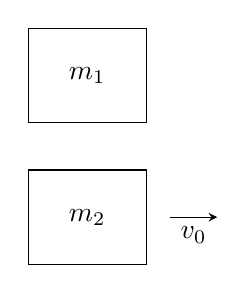
\begin{tikzpicture}[>=stealth,scale=0.6]
  \draw  (0,0) rectangle (2.5, 2);
  \draw  (0,3) rectangle (2.5, 5);
  \node at (2.5/2,4){$m_1$};
  \node at (2.5/2,1){$m_2$};
  \draw[->](3,1)--node [below]{$v_0$}(4,1);
\end{tikzpicture}
\end{document}